\chapitre{Lyre de lumière et de liberté, le lundi 10 juillet 2034 }{Erigé au début des années 70,}{ le complexe gouvernemental de Rimouski conservait son austérité d’origine, une froide sobriété tout de béton vieilli et de bois trop pâle pour faire s’épancher les cœurs, cela, malgré les rénovations auxquelles on l’avait soumis en 60 ans de services paperassiers. Au sous-sol, dans ce qui avait naguère servi de bureau régional pour le ministère de la Culture, on trouvait aujourd’hui une salle d’audience, véritable petit tribunal avec tout le décorum : drapeau du Québec, photos du premier ministre et de Sylvain Turcotte, vieux cadres numériques faisant défiler leurs scènes rupestres, forestières et maritimes, sans oublier une horloge et un calendrier électronique. On y avait entendu des promoteurs sur des histoires de prolongements routiers, des écologistes sur des questions d’enfouissement, des pêcheurs sur des enjeux de surpêche. }

Mais depuis trois mois, les locaux étaient utilisés par la Commission de réinsertion civile des victimes de la loi 173 de 2028, alias la CRC, une structure sans appel mise en place pour gommer certaines injustices survenues dans l’application de la législation Turcotte. 

Dans le cadre de la contre-réforme enclenchée dans les semaines qui avaient suivi les événements de juillet 2033, Québec avait reconnu, sur la proposition même du ministre Turcotte - une position politique déroutante que seuls quelques Rimouskois savaient forcée, le couteau sur la gorge - que certains illégaux avaient été contraints de le devenir par crainte justifiée du Bureau des affaires gérontologiques (BAG), structure policière honnie dont le démantèlement avait été terminé en janvier dernier. Ainsi, plusieurs centaines de vieillards officiellement déclarés morts avaient choisi de quitter la clandestinité pour venir plaider en faveur de leur «résurrection civile». Il leur suffisait de démontrer qu’ils n’avaient eu d’autre choix que de se cacher, traqués injustement par le BAG à la suite d’une obscure délation ou d’un discutable contrôle fiscal, la CRC leur donnait habituellement raison. À plus forte raison, que l’enquête publique du coroner actuellement en cours sur les liens pouvant exister entre chocs anaphylactiques et Nutrisuz, battait son plein avec l’attention des médias d’un peu partout, incluant ceux de la Nouvelle-Zélande et de la Suède. Et plus le temps passait, plus l’horrible soupane était décriée et pointée du doigt comme étant la cause de nombreux problèmes de santé. On s’attendait même à un recours collectif monstre dès le dépôt des conclusions à la suite des audiences. Le titre de Monsanto avait connu une chute historique.

À l’inverse, la CRC rejetait parfois les prétentions de certains demandeurs, des cas vraiment trop sulfureux pour être banalisés. Ces gens étaient alors accusés de fraude et confiés au criminel. C’est possiblement ce qui aurait pu arriver aux parents, père, mère, oncles et tantes, du gros Turcotte. Pour éviter qu’ils soient cloués au pilori et livrés à la vindicte populaire, il avait été convenu de part et d’autre, au lendemain des événements, d’offrir à ces profiteurs une nouvelle identité légale et d’en faire des résidents anonymes d’un CRG montréalais. Il ne pouvait être question de les installer dans celui de Rimouski en raison, notamment, du projet visant à le convertir en vraie maison de retraite, au grand dam de Carl Michaud, rétrogradé au rang de gérant et contrôlé dans ses moindres faits et gestes. Pour tout dire, le cadre supérieur au panache si impressionnant n’était plus que l’ombre de lui-même. En le voyant, on aurait dit un petit quincaillier en train de liquider sa faillite.

De part et d’autre ? C’est une des mesures qui avaient été négociées entre le commando dont Marie avait pris le contrôle et les gens de Sylvain Turcotte qui, sous leurs pieds, sentaient le vide sinistre de l’échafaud.

\begin{floatingfigure}[l]{45mm}

\includegraphics[height=60mm]{corps/chapitre19/img/personnage-timothee-lyre.jpg}
\end{floatingfigure}

Aujourd’hui, la salle est presque pleine. Au premier rang, Marie Rioux, Romain Tardif et leur conseiller, Robespierre Alcide. Derrière eux, le clan qu’ils ont tricoté à triple laine depuis cette fin juillet de 2033: Timothée, Béatrice, Shimoune Saint-Pierre, Ophélie Marcotte, Claude Sey qui est venu expressément de Montréal, Marie-Odile Tremblay, David Gagnon-Tropecolo, alias le Chinois, ainsi que le docteur Bellavance, Bea Bellow, Louise Lavoie, Sébastien Larose, Jipé Gendron, alias Tit-mononk, Solange Gadoury et Jawad Kebbaj, lequel, pour une fois, ne travaille pas. On remarque également quelques anciens méchants dont les frères Côté, mieux connus sous le sobriquet de Papyblues, Vlado Marcovsky, l’homme de l’informatique, et le bonhomme Jean qui avait particulièrement apprécié être libéré du sous-sol par Timothée lui-même. À un point tel qu’il lui avait «remonté» une Saguewanish grand luxe avec plus d’électronique incorporée qu’il ne s’en trouve au siège social d’IBM et avec un gyroscope dernier cri prévenant toute possibilité de chute ou de perte de contrôle gravitationnel. Une sorte de Dodge Challenger 70 avec moteur stock.

En avant, le commissaire Rémi Anglehart, celui-là même qui assumait la présidence du Centre régional gériatrique avant qu’il ne soit transformé, à la liesse générale, en résidence pour aînés, est en train de lire les considérants et s’apprête à rendre la décision ayant fait consensus auprès des membres de la CRC. La Maririou arbore son visage de pierre et celui de Romain reflète une certaine nervosité. Quant à Robespierre, psychologue officieux, colonel à la retraite et avocat autoproclamé, il sourit pour cacher son stress.

- En conclusion, la Commission est d’avis que malgré l’illégalité de l’ensemble des gestes posés, vous avez eu raison, «ab initio», de vous soustraire aux efforts des agents du Bureau des affaires gérontologiques. Leur eussiez-vous obéi, vous auriez été victimes d’une injustice encore plus grave. «Adversus periculum naturalis ratio permittit se defendere».

Anglehart se dérhume. Dans sa tête, c’est en étalant son latin qu’il arrive à se livrer à des effets de toge alors que l’instance qu’il préside n’en requiert aucune.

- En outre, poursuit-il comme s’il était à la Cour suprême, la Commission blâme le gouvernement du Québec de vous avoir contraints à l’illégalité, vous privant ainsi des services auxquels vous aviez droit, ainsi que de tous vos revenus de retraite. Il est donc de mon devoir d’invoquer un «nolle prosequi», de vous déclarer officiellement réinsérés civilement et de recommander au lieutenant-gouverneur en conseil de vous rembourser les prestations qui ne vous ont pas été versées depuis 2028, année où l’on vous a inscrits comme décédés à l’état civil, incluant, «mutatis mutandis», les intérêts que la Commission a établis à 8,367 %.

Les premiers cris de joie se font entendre.

- À l’ordre ! À l’ordre !

C’est peine perdue. Des gens accourent pour féliciter Marie, Romain et Robespierre. Le commissaire doit hausser le ton.

- Ladite Commission, crie-t-il littéralement, fera publier, d’ici dix jours, un avis dans tous les médias du Bas-Saint-Laurent à l’effet que vous, Marie Rioux et vous Romain Tardif, autrefois de Saint-Anaclet, maintenant du quartier Nazareth de Rimouski, avez, entre 2028 et 2034, agi «bona fide», que vous avez été réinsérés aux dépens de l’État, que vous avez bel et bien été victimes d’une loi mal appliquée et, «res ipsa loquitur», que vous recevrez les excuses formelles du gouvernement du Québec.

À ces mots, la salle explose comme à un match de football. Anglehart n’a jamais rien vu de tel. Claude Sey a les larmes aux yeux, Tropecolo lui serre les deux épaules de ses courtes paluches, Jawad Kebbaj donne l’accolade à Timothée, Ophélie fait la bise à Shimoune, Bea Bellow sourit et, l’espace de deux secondes, frotte ses jointures de la main droite sur l’avant-bras de Robespierre, imitée par Louise Lavoie qui elle, embrasse carrément le colosse sur la joue, ce qu’observe Marie-Odile, la nouvelle responsable de la sécurité, qui lorgne la scène du coin de l’œil par crainte inavouable qu’on lui pique l’homme de sa vie, son beau Robie. Au même moment, Tit-mononk lève un spectaculaire bras d’honneur en direction de la photo du premier ministre sous les rires de Marcovsky et sous la mine ravie, celle des grands jours, de Sébastien Larose qui venait tout juste de prendre sa retraite. Le père Jean, lui, file sur la Saguewanish Hot Rod prétextant un dernier ajustement. Quant au docteur Bellavance, homme de science auquel plus personne n’accole l’épithète de «sinistre», il gagne discrètement la sortie, un sourire accroché au visage, suivi de Solange Gadoury qui semble ne plus vouloir le quitter depuis qu’il mène un projet de reconditionnement nutritionnel destiné aux cas de patients ayant développé une intolérance pathologique à la nourriture en raison des abus de Nutrisuz. Jamais sa vie n’a été aussi intéressante.

À son tour, l’arrière-petit-fils de l’inventeur du Pétépano s’approche de Marie.

- On les a eus, madame Rioux ! Et dans l’honneur ! Ils vont même vous faire des excuses publiques. Vous allez pouvoir marcher en plein jour, dans les rues de Rimouski, au su et au vu de tout le monde. Vous avez réussi à faire travailler notre matériel, nos preuves. Avec ça, ils ont tous plié. Ils vous ont donné tout ce que vous exigiez.

- Voyons, mon garçon, tu sais aussi bien que moi que dans cette histoire, je n’ai joué que ma partition et que chacun a joué la sienne. Sinon, ça n’aurait pu fonctionner.

Robespierre Alcide qui a tous les talents avec les dames, lui fait alors une profonde révérence.

- Et si on n’avait pas eu une bonne chef d’orchestre, ça n’aurait pas pu fonctionner non plus !

Le lendemain de l’opération commando, Marie avait effectivement exigé la présence de Sylvain Turcotte dans son salon, au sous-sol de la rue Crouet. Louis-Marc Richard n’en était pas revenu de voir autant de voitures, dont celle du ministre rimouskois, arriver chez son voisin d’en face, ce «pas d’allure» hautement suspect. C’est avec la plus tordue des fiertés, qu’une Maririoux aussi rigide qu’implacable avec reçu le haut personnage, assise dans son fauteuil crevé, laissant Gazou essayer de mordre les mollets libéraux qui s’aventuraient trop près de sa méchante gueule. La vieille dame avait exigé la présence de Romain, Timothée, Shimoune et Robespierre et, en contrepartie, avait accepté que quatre sbires accompagnent l’homme politique. D’entrée de jeu, elle avait voulu comprendre pourquoi le politicien avait fait basculer sa famille dans l’illégalité. N’avait-il pas les moyens, lui, «un gros ministre pesant», de subvenir aux besoins de son père et de sa mère pour leur éviter, en toute légalité, l’internement dans un CRG ?

La réponse ne l’avait pas ébranlée du tout. Quand il avait vendu sa terre pour prendre sa retraite en 2028, l’année du référendum, le gros Jean-Pierre Turcotte n’avait, en réalité, que poussé des feuilles de papier. Hypothéquée jusqu’au trognon, la propriété agricole ne lui avait presque rien retourné en équité. Lui-même criblé de dettes, le cultivateur rimouskois s’était retrouvé sans le sou, avec Mimi qui s’assurait, sur une base quotidienne, que la vie soit vraiment invivable. Pour tous revenus, le couple disposait de la pension fédérale et de l’allocation provinciale, celle de la Régie des rentes. De plus, Sylvain leur avançait quelques centaines de dollars tous les mois, la plupart du temps pour payer le loyer de leur 4 ½, rue Saint-Jean-Baptiste. En échange, ils l’aidèrent sérieusement, tous les deux, dans sa campagne référendaire.

Une fois la loi 173 adoptée, les deux Turcotte auraient dû, techniquement, être forcés d’aller habiter au CRG-BSL. C’est à ce moment que Mimi eut l’idée de faire construire un pavillon au Bic et de disparaître avec Jean-Pierre pour mieux s’y cacher. Elle en profita pour offrir cette chance unique à ses deux sœurs et à leurs époux. Sylvain Turcotte fit le nécessaire à la satisfaction générale. D’où le terrible accident de juin 2029.

- Faut me comprendre, ma’me Rioux, j’ai une famille à m’occuper ! P’is une paye de ministre, ce n’est pas une paye de président de compagnie. C’est pas assez pour faire vivre mes parents en même temps que ma femme et mes enfants; j’en ai deux au cégep et un à l’université. Ma femme, vous l’avez connue dans l’temps, elle a pas changé, elle est malade tout le temps, elle travaille pas, elle rapporte rien, c’est toute moi qui paye toute, tout le temps.

La vieillarde avait alors frappé l’accoudoir de son fauteuil, ce qui avait momentanément calmé Gazou.

- Cha va faire, j’en ai achez entendu; tu me feras pas brailler chur ton chort, mon ‘tit garchon. T’es «quelqu’un de pouvoir» qui m’a trahie !

C’est à ce moment que la Maririou, le visage intraitable, avait placé ses cartes : voici les preuves de corruption, voici des preuves de faux déposés au Conseil d’administration, voici des preuves vidéo où le ministre des CRG cache des illégaux, en l’occurrence sa parenté, et voici des preuves démontrant, hors de tout doute, que des vieillards sont maltraités et emprisonnés. Tout ce petit matériel a été stocké dans différents systèmes informatiques pour éviter qu’il ne soit détruit. La seule façon qu’il y reste verrouillé à quadruple tour, qu’il ne soit ni envoyé aux médias, ni remis à la police, ni téléversé dans le quanticordi de Thierry-Ian Dennis-Dubeau, le chef de l’opposition à Québec, c’est que l’on procède rapidement à quelques petits changements.

Petits changements ! Quel euphémisme !

- Mon ‘tit garchon, j’te donne un an pour faire tout che que je vais te demander. Chi tu y arrives pas, t’es dans la misére !

- Ma’me Rioux …

- Pour t’aider, avait-elle coupé, je l’ai tout écrit ichi sur che document. Y en a une copie pour toi et une pour moi que tu vas chigner. Si tu chignes pas, demain matin neuf heures, les médias, la poliche et Dennis-Dubeau, tu chais, Ti-Dédé, b’en ils vont rechevoir toutes les preuves. J’ai quelqu’un qui m’a toute arrangé cha pour que cha parte.

- Ma’me Rioux, ma’me Rioux, vous savez bien que c’est pas comme ça que ça marche. Va b’en falloir que je prenne le temps d’étudier vos demandes. Après, on se rencontrera et on verra ce qui peut être fait.

- Ch’est comme tu veux. Chi tu chignes le papier, tu gardes ta job, chi tu chignes pas, demain matin neuf heures, t’es dans la pire misére noire de toute ta vie ! Y a rien à négochier, abcholument rien, mon pauv’tit garchon ! T’as été malhonnête, tu t’es fait pogner, à ch’t heure, tu paies. À ma fachon ! Chinon, ch’est la prijon, le déjhonneur, le pipi dans les claques.

Bluffeur notoire, Turcotte avait alors fait mine de sortir, les trois janissaires à sa suite. C’est à ce moment que Robespierre avait mis en marche son vieux fond Alcide.

- Êtes-vous au courant, monsieur Turcotte, de la situation sordide dans nos prisons depuis qu’il y a quatre ans, votre régime a sabré de 40 % dans les budgets correctionnels ? Les autres détenus vont tellement vous tabasser que je n’aurai pas besoin d’aller vous porter de caramels, vous n’aurez plus de dents pour les manger et vos lèvres seront des enflures crevassées, des horreurs indicibles.

- Et, avait ajouté le malicieux Shimoune, j’aime autant pas parler de l’état de votre pauvre anus.

Il s’en était suivi une engueulade mémorable au terme de laquelle, vingt minutes plus tard, le gros Turcotte s’était assis et avait commencé à prendre connaissance des demandes du commando.

- Timothée, tu lui echpliques, moi, j’ai p’us vraiment le goût d’le faire !

Et elle avait allumé la télé et s’était mis les écouteurs.

- Monsieur le ministre, avait continué le fils, papelard en main, si vous le voulez bien, euh … je vais vous lire nos 25 exigences non négociables, telles que formulées par ma mère et endossées par nous tous. Vous avez le même document que moi. Euh, je lis, c’est à la page 1 :

    Article un : Tout sera mis en œuvre pour que Marie Rioux ait accès, dans les plus brefs délais, aux services d’un dentiste afin qu’on lui fabrique des prothèses, ce qui lui permettra de parler sans chuinter.

- Euh … elle y tient beaucoup, avait dû ajouter l’inimitable Timothée devant l’incrédulité de l’homme fort du pari libéral.

Quant aux 24 autres articles, ils avaient été lus sans aucune réaction de Turcotte. On aurait dit qu’il écoutait la fatalité lui dicter son arrêt de mort et la méthode détaillée de son exécution. Selon le consensus désordonné auquel était parvenu le comité «Bec-mord», patronyme découlant de BCCMMORRST, pour Béatrice, Christian, Claude, Marie, Marie-Odile, Robespierre, Romain, Shimoune et Timothée, un consensus plein d’espoir, un tantinet idéaliste et, dans l’ensemble, pratico-pratique sur lequel n’avait peiné, c’était évident, aucun disciple de Thémis, on commençait, d’entrée de jeu, par exiger que la pratique des cérémonies de groupe, avec mise à mort des malades, soit immédiatement abolie sur le territoire du centre rimouskois. En même temps, on déclarait que l’inique Bureau des affaires gérontologiques, alias la police des vieux, n’avait plus juridiction dans la région administrative du Bas-Saint-Laurent.

Puis, on «ordonnait» que le CRG-BSL soit transformé, dans les plus brefs délais, en résidence pour personnes âgées, en maison de la culture ouverte sur toute la communauté régionale et en centre de recherche gérontologique affilié à l’Université du Québec à Rimouski, l’UQAR. Pour y arriver, précisait-on, un projet pilote devait être enclenché au plus tard le 1er août. En corollaire, les aînés du Bas-Saint-Laurent n’étaient plus contraints d’y être hébergés. Mais ceux qui le voulaient le pourraient dès que les réaménagements nécessaires auraient été complétés; ces gens seraient alors considérés comme locataires. Il va sans dire que les notions de salles 2P, 3P et palliatives étaient abolie. Il n’y aurait ainsi plus de dortoirs, plus d’ailes nord, centre et sud. Des équipes de rénovateurs feraient de ces salles des chambres pour personnes seules, pour personnes en couple, voire en famille, pour retraités plus fortunés, sans oublier de petites boutiques de dépannage. Des tarifs et du financement seraient imaginés et implantés. Quant au Centre nutritionnel, le comité le transformait en véritable réfectoire ou cafétéria et les machines à Nutrisuz étaient envoyées à la casse. Seule de la vraie nourriture saine serait dorénavant servie.

- On niaise pas avec ça, avait précisé Shimoune. C’est une des premières choses qu’on va faire. On va même recruter du personnel professionnel. Bye-bye Amédée Chicot ! Quin mon cochon !

- S’il te plaît, Shimoune, laisse-moi lire le document au ministre.

En ce qui a trait à l’inquiétant centre de recherche hormonal du sous-sol, il serait réaffecté, dans les plus brefs délais, en entité d’étude sur la réadaptation alimentaire des personnes âgées qui, au cours des trois dernières années, n’avaient mangé que du Nutrisuz. Ici, il était stipulé qu’en plus d’une équipe de chercheurs, il y aurait une collaboration avec l’Université du Québec à Rimouski (UQAR). En outre, un centre de santé avec médecins, personnel infirmier, équipement moderne et ambulance pour transfert éventuel vers l’hôpital de Rimouski, serait créé. Les professionnels de la santé seraient tenus de visiter régulièrement tous les résidents. Ici aussi, il y aurait partage structurel avec l’UQAR.

- Le comité – Timothée pensait plutôt à Béatrice qui avait fait ajouter ces points – a de bons contacts à l’université et, s’il le financement ne tarde pas, ça sera assez facile d’organiser ça.

Dans la logique de la rénovation, la salle du Conseil d’administration se transformait en bibliothèque avec ressources humaines compétentes et, stipulait-on dans le document du comité «Bec-mord», des livres en quantité suffisante devaient être achetés. Le salon du personnel, lui, il était déménagé dans la partie sud de la cafétéria et une cloison était érigée pour en faire une pièce séparée avec accès directement du couloir. En lieu et place, l’espace ainsi libéré était retourné à sa vocation d’origine, c’est-à-dire un gymnase. Sous la responsabilité du directeur des loisirs Robespierre Alcide, des équipements modernes d’intérêt gérontologique étaient achetés et des employés spécialisés étaient embauchés. Il va sans dire que la piscine du sous-sol était remise en fonction.

L’article suivant était suave.

    Article 13 : Les actuels préposés aux bénéficiaires verront leur définition de tâche considérablement changée. Ils ne seront plus en situation d’autorité sur des patients, mais en situation de services auprès de locataires. Ils seront des aidants, où, notamment, ils devront offrir des services d’écoute, de courses, d’entretien, de réparation, d’accompagnement ici et là, incluant à l’extérieur dans la région.

- Ça mon ami, ce ne sera pas évident. Pense à toutes les crapules que l’on côtoie. Va y avoir un méchant ménage à faire !

- Laisse-moi continuer, Robespierre. Monsieur Turcotte a un emploi du temps très chargé.

Le fils Tardif avait alors abordé les questions relatives à la Sécu, laquelle - on sentait ici l’influence de Marie-Odile - voyait ses effectifs coupés de moitié. Tous ses systèmes d’espionnage, d’écoute ou de captation se retrouvaient réduits au niveau toléré dans les endroits publics du Québec. En prime, on décrétait que le centre d’incarcération du sous-sol était transformé en atelier de réparations avec du personnel spécialisé, du «personnel empathique», était-il précisé.

- Bye-bye les Papyblues !

- S’il te plaît, Shimoune !

Tout cela, bien entendu, ne pouvait se faire que si les lettres patentes de la corporation du CRG-BSL étaient temporairement abrogées, le temps du déroulement du projet, que si le Conseil d’administration du CRG-BSL était suspendu sine die et remplacé par un comité de coordination, une structure opérationnelle fonctionnant par consensus un peu comme le comité «Bec-mord», que si le personnel de la direction générale était réduit de moitié et que si le grand patron était nommé «gérant».

Le plaisir évident avait un peu fait trébucher Timothée sur les deux articles suivants :

    Article 19 : À des fins d’efficacité et pour optimiser les chances de réussite dudit projet, M. Carl Michaud, actuellement directeur général du CRG-BSL, sera destitué de ses fonctions et embauché aux deux tiers de son salaire actuel, comme gérant avec contrat de trois ans, terme au cours duquel il lui sera formellement interdit de démissionner. À défaut de se soumettre à la logique de cet article, il devra répondre de ses actes passés.

    Article 20 : La direction des communications sera abolie et la tâche sera confiée à un employé dans l’entourage du gérant.

- Dans les dents, mon Flipper ! Quin, mon Carl !

- Shimoune, tais-toi !

La partie plus culturelle du consensus «Bec-mord» témoignait de l’influence de la Maririou. On apprenait, en effet, que tous les bureaux administratifs de l’établissement seraient relégués à l’extrémité nord du rez-de-chaussée et que le reste de cet étage, ainsi qu’un grand secteur du sous-sol, notamment le local d’entreposage mortuaire et d’incinération que l’on convertissait en petite salle de spectacle, seraient affectés à la deuxième vocation de l’édifice, la culture. Et, comme il se doit, l’École populaire de musique, «lâchement abandonnée par l’État en 2021», se voyait relancée dans ces nouveaux locaux avec financement garanti par Québec pour au moins dix ans et embauche d’employés qualifiés. Quant au public cible, il serait de tout âge, un public provenant de la communauté régionale. Il était en outre précisé qu’il fallait s’attendre à ce que d’autres initiatives culturelles soient lancées au fur et à mesure de l’avancement du projet: multimédia, peinture, écriture, théâtre, etc.

Une fois l’immense tâche menée à terme, soit le 31 juillet 2034, «c’est dans un an d’ici», elle sera évaluée à son juste mérite et advenant que cette méga réforme soit une réussite, elle se verra implantée ailleurs au Québec selon des modalités à être établies. Il va sans dire que la législation québécoise sera modifiée en ce sens.

- Ça veut dire, monsieur Turcotte, que la notion d’illégaux, ces vieux qui vivent actuellement cachées, sera revue et ces gens, décriminalisées.

- J’y arrivais, Robespierre.

L’article 24 prévoyait, en effet, qu’il incomberait au gouvernement du Québec de créer un mécanisme permettant de réintégrer dans la société des personnes ayant été contraintes de devenir, par la force des choses, illégales à partir de l’entrée en fonction de la loi 173 de 2028.

- À vous de réparer vos injustices !

En entendant la lecture de l’article final, article où le sarcasme cohabitait avec la menace, l’énorme politicien n’avait pu contenir sa colère.

    Article 25 : La maîtrise d’œuvre et le financement de cette réforme seront confiés au ministre des Affaires gérontologiques, vice-premier ministre du Québec et député de Rimouski, l’honorable Sylvain Turcotte, afin qu’il puisse voir le parcours de sa carrière se continuer dans l’harmonie.

- Êtes-vous malades, avait alors explosé l’homme fort du parti libéral ? Vous pensez vraiment que c’est moi qui va s’occuper de vos folies, gang d’amateurs ? Trouvez-vous un autre cave !

- Le cave, on l’a, p’is c’est toi, mon gros verrat.

Romain s’était alors approché à deux pouces de l’immonde pif couperosé. Ce qui avait créé un mouvement ondulatoire dans la masse des quatre attachés, dont une avocate de Montréal qui tentait de calmer le ministre.

- M’a t’en faire, espèce de vieux malpoli !

- Ta gueule Turcotte, p’is écoute-moi comme i’faut ! Le jour où tu vas décider de boquer, de ne pas nous obéir, ça va être «clic, la prison» ! C’est moi ici, Romain Tardif, qui va peser sur le piton, as-tu compris ? Et là, en dedans de dix minutes, crac !, les médias, la police et Ti-Dédé vont recevoir toutes les preuves qui faut pour te faire pendre, mon gros chie-en-culotte! P’is à part de ça, avise-toi pas de démissionner; fais rien qu’y penser et moi je fais clic ! As-tu compris ? À c’t heure, ch’naille, j’t’ai assez vu !

Furibond, Turcotte s’était levé en balbutiant de vagues menaces. Mais Timothée s’était interposé avec sa copie du document.

- Papa, attends ! Faut qu’il signe s’il veut pas se ramasser en prison.

Capté par trois caméras différentes, le ministre avait alors griffonné sa signature avec une vigueur à déchirer le papier et à égratigner la table. Puis il était disparu dans l’escalier, suivi de son personnel politique et de Timothée. En bas, dans le salon, Robespierre, Romain et Shimoune s’étaient mis à rire comme des écoliers qui venaient d’échapper aux griffes du directeur.

- Marie, avait chantonné le bonhomme en enlevant un des écouteurs à sa compagne, il a signé le gros pourri !
Mais la vieille avait alors haussé les épaules et s’était rebouché l’oreille.

- Fallait b’en manque qu’i’ chigne ! Y était cuit !

\begin{floatingfigure}[l]{55mm}
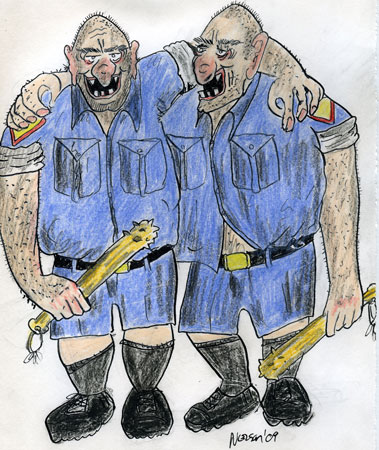
\includegraphics[height=60mm]{corps/chapitre19/img/personnage-papyblues.jpg}
\end{floatingfigure}

Le lendemain, alors que Timothée, toujours privé de son dispositif personnel polyvalent et de sa Saguewanish, était descendu au sous-sol du Centre faire libérer le père Jean, il s’était également occupé des deux frères Papyblues. Que leur reprochait-on, au juste, à ces malabars ? D’être grands, musclés, laids, bêtes, dangereux, terrifiants, d’avoir les dents sales, les ongles noirs, la mâchoire à figer le sang et d’appliquer, sans questionnement, les directives qu’on leur signifiait ? Avaient-ils déjà tabassé des bénéficiaires ? Non ! Avaient-ils déjà torturé des prisonniers ? Pas plus ! Avaient-ils déjà cloué des chats, provisoirement vivants, sur les portes de leurs geôles ? Que nenni ! Avaient-ils déjà coupé des rats en fines lamelles pour faire cuire un chow mein ? Encore moins ! Avaient-ils déjà dévoré de petits enfants, en commençant par la tête ? Absolument pas ! Le CS-1 leur avait fait alors une proposition de recyclage. De deux choses l’une, soit que les méchants gagnent, soit qu’ils perdent, et, advenant le deuxième cas, il y aura un important ménage. Un ménage de fond en comble.

- Si vous marchez avec nous, vous gardez votre job. En cas contraire, vous vous retrouvez, d’ici un mois maximum, sur la terre paternelle, dans l’arrière-pays. Donc, vous faites quoi ?

L’un des frères Côté avait grimacé un rictus à faire frémir le plus redoutable des gladiateurs du cirque Maxime sous l’empereur Trajan.

- On n’est pas con, chef ! On t’a vu aller. On sait qu’il y a ceuze pour qui les patates sont collées au fond, p’is qu’y a ceuze pour qui le party est à veille de pogner. Nous autres, on aime ça les partys !

Timothée avait alors souri et avait tendu la main. En l’écrasant, sans aucune malice, les deux Papyblues étaient devenus les gardes du corps de Marie et Romain. En poste 24 heures sur 24 chez Timothée, ils faisaient en sorte que le pire des scénarios, celui selon lequel Pete Barrett s’en prendrait aux personnes du couple Rioux-Tardif pour tenter de désarmer le groupe, s’avérerait désormais impossible. Sauf, qu’ils bâfraient comme des déchaînés et Timothée devait mettre ses amis à contribution pour renflouer ses armoires. Consulté sur cette importante question de sécurité, le colonel Alcide et son adjointe l’adjudant-chef Tremblay, une adjointe de plus en plus … intime, avaient averti tous les autres membres du comité «Mord-bec» d’être extrêmement prudent et, quand ils se retrouvaient seuls, de toujours avoir leur DPP en mode captation vidéo. Heureusement, un événement lourd de conséquences était venu régler le problème logistique causé par la goinfrerie des Papyblues.

En annonçant le projet pilote et les mesures soi-disant temporaires qui l’accompagnaient, le ministre Turcotte était devenu, pour les uns, une sorte de héros, un homme de compassion, de cœur, de sentiment, un personnage public honnête qui reconnaissait avoir peut-être commis des erreurs avec sa loi 173, un humaniste pour qui le bien-être et la dignité des aînés primaient sur la performance budgétaire de l’État et sur sa carrière politique. Pour les autres, il était ce qu’il avait toujours été, un politicien tirant la poche de son bord, c’est-à-dire du côté de son électorat rimouskois, des régionaux très éloignés de Montréal qui, les veinards, bénéficiaient d’un régime humanitaire exceptionnel. Quoi qu’il en soit, en une semaine, si on en croit les sondages et les vox-pop, il avait dépassé Ti-Dédé dans l’estime populaire et était de loin, la personnalité québécoise la plus admirée. Les éditoriaux l’adulaient, les talk-shows se l’arrachaient, les corps intermédiaires s’organisaient pour que dans leurs régions, la même chose se produise, il était invité partout où il y avait une plateforme. Même sur l’île d’Anticosti, la colonie de vieux squatters commençait à donner signe de vie et à communiquer avec l’entourage de l’homme politique. Avec l’âge, certains résidents semblaient préférer être rapatriés sur le «continent».

Sa gloire était telle qu’il s’était pris à son propre jeu et, en un mois, était devenu franchement convaincu qu’il fallait aller dans le sens des revendications du comité «Mord-bec», ce qui avait frustré bon nombre de profiteurs du régime. En fait, Turcotte s’était retrouvé tellement imbu de sa nouvelle importance et de son enviable réputation, qu’il avait juré aux parents de Timothée, un jour où la Maririou l’avait à nouveau convoqué sur la rue Crouet et qu’il s’était inquiété de la présence des sinistres frères Côté, que jamais au grand jamais, il n’accepterait, ni ne couvrirait, ni ne tolérerait toute exaction, violence ou autre vexation commise à leur endroit ou à celui de leurs amis, cela articulé solennellement devant trois caméras et quatre témoins. Il avait été tellement convaincant que peu après, les Papyblues avaient été retournés au Centre pour aider aux innombrables transformations en cours.

Au fil des mois, le projet avait pris corps. Confirmé dans sa tâche de directeur des loisirs, Robespierre avait tout de go commencé à en mener large avec l’aménagement du gymnase et de la piscine, dont il avait confié la responsabilité à son adjoint de fraîche date, Shimoune Saint-Pierre. «Tu viens faire splish splash avec moi, mon beau Robie ?» L’héritier du Pétépano avait également dû se dépêcher de nommer Bea Bellow responsable de la transformation de la salle du CA en bibliothèque. La vieille dame ne se souvenait pas d’avoir été aussi heureuse dans sa vie. Quant à Louise Lavoie, elle pouvait à peine l’aider, aux prises elle-même avec une collection quotidienne d’ennuis matériels défiant l’imagination la plus débridée.

La veille du début des travaux visant à en refaire un gymnase, le salon du personnel avait servi à recevoir la quasi-totalité des employés où l’ancien commando du 29 juillet 2033 qui s’était octroyé la totalité des sièges au comité de coordination avait répondu à toutes les questions et expliqué toutes les conséquences du changement d’orientation de l’établissement sur les postes. Si plusieurs demeuraient inchangés, de nombreux disparaissaient et d’autres étaient à combler, par exemple en alimentation, en entretien ménager, en loisirs, en soins infirmiers, en assistance gériatrique, en encadrement de bénévoles et ainsi de suite. Les intéressés n’avaient qu’à se manifester. Tous ceux qui voulaient conserver leur lien d’emploi étaient les bienvenus. Mais ils devaient méditer sur le fait que toute forme de malhonnêteté, d’abus, d’extorsion, de manquement éthique, de violence, physique ou verbale, et autres turpitudes à l’endroit des bénéficiaires, ou des locataires comme on les appellerait sous peu, serait immédiatement sanctionné par un congédiement sans appel avec rapport détaillé sur le certificat de licenciement.

Dans les deux mois qui avaient suivi, plus de 35 % des effectifs avaient choisi de partir, dont plus de 70 % des chefs de section et des cadres. «Bon débarras !» s’était écrié le colosse en apprenant la démission du gros Lavoie et du redoutable Pierre Monger, ex CS-1 du 4e Sud. En revanche, le départ de Claude Sey voulant retourner à l’université compléter un doctorat en ethnologie, l’avait profondément chagriné, tant il appréciait l’honnêteté et l’idéalisme altruiste du jeune homme.

Côté informatique, Vlado Marcovsky avait décidé de rester en poste et, à la demande du Comité, avait fait table rase de l’erratique système panrégional pour en implanter un nouveau entièrement basé sur du logiciel libre. Une enquête avait démontré que le diagnostic posé peu avant sa mort par Pierre Asselin, un vieil ingénieur quasi aveugle placé sous la responsabilité de Timothée, avait été juste. Il y avait effectivement eu tatouage de puces. Marcovsky et son équipe avaient eu besoin de quatre mois, incluant le temps de débogage, pour tout refaire. Il est vrai qu’il n’y avait plus de bénéficiaires à gérer, par contre les projets de recherche, en raison de l’implication de l’université et des travaux du docteur Bellavance, abondaient.

Pendant ces mois fébriles, rien n’était plus drôle que de voir Robespierre entrer, sans jamais frapper, dans le coqueron mal aménagé – merci Louise Lavoie - qui servait d’officine au gérant Carl Michaud pour lui faire signer des documents qu’il lui interdisait de lire. Amaigri, accablé, la peau grisâtre, l’ancien DG semblait au bord de la dépression. Dans les premiers temps de son calvaire, il avait essayé de plaider la cause de Philippe Dauphin. Mais le comité de coordination avait rejeté la demande. Flipper avait été bouté hors de la région avec promesse que si jamais on entendait à nouveau parler de lui, on le traquerait et on l’offrirait en pâture aux Papyblues. Il avait ensuite tenté sa chance avec Amédée Chicot sans plus de succès. On lui avait alors garanti qu’advenant que l’on retrouve cet abominable personnage, on en ferait une attraction populaire en l’enchaînant à vie, dans une cage bien en évidence au rez-de-chaussée du nouveau Centre, avec, pour nourriture exclusive, du Nutrisuz à saveur de poutine aux similis bacon.

Lentement, tout au long d’août et septembre 2033, la plupart des pensionnaires avaient été déménagés soit dans les familles, soit dans des hôpitaux, en attendant que les travaux soient complétés. Robespierre n’avait plus été sollicité pour des pilules du bonheur. Ceux qui avaient choisi de rester au Centre avaient été relogés temporairement au dernier étage, territoire naguère terrifiant qui venait de se transformer en colonie de vacances pour vieillards n’ayant nulle part ailleurs où aller, dont l’éprouvant Jean Saint-Gelais, le tandem aux mœurs discutables Thériault – Labbé et Luce Morency.

- Madame Thériault, vous seriez gentille d’avoir un œil bienfaisant sur madame Morency, avait demandé Timothée, désormais responsable de la dizaine d’employés affectés à cet étage. Il lui arrive de fuguer…

- J’me souviens d’elle au lac Saint-Mathieu. Belle femme, la Luce Morency …

- Moi aussi je me souviens, madame Thériault, moi aussi.

- J’vas m’en occuper, chef, fais-toi-z-en pas. J’y ferai pas mal !

- Profitez-en, vous et madame Labbé, pour vous installer dans la «p’tite chambre» de l’ancienne aile sud, à l’autre bout. Y a personne dedans. Vous allez avoir euh … la paix. En tout cas pour un bout de temps.

- Ça te dérange p’us qu’on soit gouines ?

- Ça ne m’a jamais dérangé, madame Thériault.

L’ex CS-1 avait à peine eu le loisir de s’approcher des ascenseurs que la vieille Loubert l’avait interpellé.

- B’en beau vos réformes, chef, mais moi je n’ai plus de sacs depuis une semaine. Vos gars, ici sur l’étage, ils savent pas où en trouver.

- Je m’en occupe, madame Loubert.

Une heure plus tard, Timothée réapparaissait avec une lourde caisse contenant de quoi satisfaire la victime de colostomie pour au moins un an.

C’était il y a dix mois, alors que tout était à faire. Aujourd’hui, dans cette salle d’audience trop climatisée, compte tenu des froides averses qui s’abat sur l’Est-du-Québec depuis près d’une semaine, Timothée qui n’entend plus rien, regarde tous ces gens qui, autour de lui, s’affichent ouvertement fous de joie, la plupart ayant attendu à la dernière minute pour lever un petit doigt d’appui. Heureusement, certains ont mérité d’être de la fête. Ici, Shimoune avec son ami de cœur, un ergothérapeute récemment embauché, là, Robespierre tenant Marie-Odile par la taille. Plus loin, Claude Say en séance de congratulation en compagnie du vieux Romain, encore plus loin, Béa Bellow et Louise Lavoie en train de rire aux éclats avec les frères Côté, près d’elles, Mmes Thériault et Labbé encadrant Luce Morency qu’elles ont vêtue d’un tailleur marine et dont elles ont coiffé les longs cheveux en chignon 1900, puis, à quelques mètres à sa gauche, Béatrice, SA fille sous la lanterne, occupée à converser en toute gentillesse avec un couple de médecins fraîchement recrutés et diplômés de l’Université de Montréal, deux jeunes idéalistes venus prêter main-forte à la contre-réforme du gros Turcotte. «Allez Béatrice, rends-les accrocs de ton charme !» Embauchée par l’UQAR, elle assumait depuis quelques mois la coordination des activités en recherche-action gérontologique et gériatrique que déployait le centre de haut savoir.

\begin{floatingfigure}[l]{40mm}
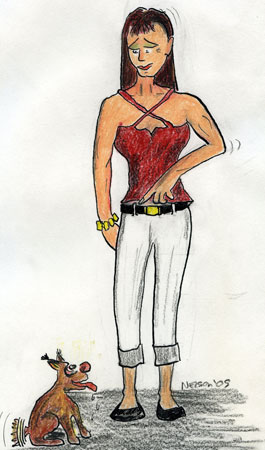
\includegraphics[height=60mm]{corps/chapitre19/img/personnage-beatrice-gazou.jpg}
\end{floatingfigure}

Quand leurs yeux se croisent enfin, le sourire de l’infirmière change aussitôt de registre. De socio-amical qu’il était, il devient beau, irrésistible, brûlant, amoureux. Partout, dans chaque capillaire de Timothée, dans chaque cellule de sa peau, dans chaque atome de tissu, une sensation enveloppante de bonheur, de chaleur, d’attraction, d’émotion, vient investir toute la place organique. Ce qu’il contemple alors, ce qu’elle le voit contempler avec une telle ardeur, ce n’est pas seulement une de ces femmes de rêve, «solitaire dans la foule comme en forêt», une de ces «femmes d’espoir heureux» telles que chantées naguère, des femmes que l’on mérite «en restant libre». Non. Ce qu’il voit, c’est cette femme qu’il vénère à chaque instant, cette femme qui, depuis près d’un an, le rend heureux le matin, le midi, le soir, la nuit, cette femme qui lui a fait oublier, revoir, réorganiser, repenser, 44 ans de vie pas toujours facile, une vie de gras du bide chauvasson et barniqueux. Il doit s’approcher, étirer l’instant de vertige, il lui faut aller goûter cette source d’apaisement, il doit aller entremêler son aura dans celle, toute en douceur enveloppante, de Béatrice. Plus rien ne peut le retenir.

- Timothée, viens, faut que j’te parle.

C’est la Maririou.

- Viens voir, j’ai quelque chose à te donner.

Un peu pour faire contre mauvaise fortune bon cœur, Timothée s’extirpe lentement de son envoûtement et suit sa mère qui navigue dans la foule comme une mamie impavide brandissant un terrible parapluie. La porte franchie, elle entre dans un grand vestiaire et, sur une tablette en haut des cintres, prend un sac de jute, une de ces poches dans lesquelles, à Saint-Anaclet, elle conservait d’innommables produits de son jardin.

- Là, ton père p’is moi, ils viennent de nous ressusciter légalement. Ça veut dire deux choses pour moi. Un, je deviens directrice de l’École de musique et on commence demain matin. Deux, je débute comme directrice musicale d’un orchestre de chambre et on donne un premier concert dans six semaines. Ça fait trois mois que je recrute des musiciens en cachette. On est rendus à 27, de tous les âges, et la plupart ont un passé professionnel. Ton père va même y être clarinettiste.

Timothée a pâli.

- Mais moi, je vais me contenter de diriger, je ne suis plus une bonne violoncelliste. Mes vieux doigts ne suivent plus. P’is toi, mon tit garçon, rassure-toi, je ne veux pas que tu en fasses partie avec ton cuivre à coulisse. N’aie pas peur ! T’as jamais aimé cet instrument et tu en as toujours joué parce que c’est moi qui l’exigeais, pour me faire plaisir, pour m’obéir, pour que je te foute la paix …

- Euh …

- … ou, peut-être, pour que je m’intéresse à toi.

Son regard fixant les portes de la salle, elle lui tend le sac.

- Tiens, c’est pour toi.

Timothée s’en empare et y enfouit son avant-bras où il découvre un étui en tissu capitonné un peu plus étroit, mais à peine, que celui de son trombone.

- C’est quoi ?

- Ouvre, tu vas voir ! Ça vient du Pays de Galles, c’est fabriqué par un artisan et on me l’a livré hier. C’est quelque chose qui va peut-être t’aider à te trouver, toi, un être libre que sa vieille folle de mère a trop longtemps essayé de modeler à sa façon, ce qui t’a empêché, pauv’ tit garçon, d’être dans la vie ce que tu étais dans ton petit cœur. J’ai tout compris ça en me débarrassant de la haine, de la peur, de la rage que j’éprouvais constamment à cause de mon père. La paix m’est venue, comme ça, après avoir réglé son cas au gros Turcotte, en lui arrachant les dents. J’ai pu tuer ma rancœur, étouffer ma maladie, pisser tout mon vinaigre.

Incrédule, inquiet, impressionné, curieux, le fils ouvre l’étui et y découvre une lyre.

- Une lyre ?

- Une lyre Sutton Hoo, mais à sept cordes, le même symbole de lumière et d’harmonie que la lyre dont jouait Timothée de Milet, le Grec qui a changé la musique pour éviter qu’elle ne le change, lui. Un homme qui avait compris que la vie, il fallait la vivre à sa façon et non à celle des autres, incluant, probablement, sa mère.

Les mots ne viennent plus à Timothée, embouteillés, qu’ils sont, dans un goulot bien étanche.

- C’est ton instrument, maintenant.

Et elle le gratifie d’un des rares sourires en 83 ans de parcours, un sourire si beau qu’il en ressent un grand bien-être. Puis, elle lui tapote doucement l’épaule et s’en retourne, de son trot de petite vieille pressée, vers l’intérieur de la salle d’audience.

- Apprends à en jouer, lui crie-t-elle avant de disparaître.

Penaud, les yeux rivés sur la lyre, il est figé, incapable d’exprimer quoi que ce soit. Béatrice qui avait observé la scène s’approche pour le tirer de sa catatonie.

- Viens, Timothée, on s’en va chez nous.

Dans le taxi de Jawad Kebbaj, avec son bouleversant cadeau sur les cuisses et un feuillet d’instructions en main, il dira :

- C’est diatonique, do, ré, mi, fa, sol, avec les deux cordes d’extrémité en la.

Puis, devant la maison de la rue Crouet transformée, depuis l’arrivée de la belle infirmière, en cottage coquet décoré d’arbustes, de fleurs et de rideaux, gratifié d’une peinture récente ainsi que de volets neufs et complété d’une clôture aussi inutile que mignonne, il ajoutera :

- Ce qu’elle vient de me donner, maman, ce n’est pas une lyre, mais la liberté. Ma liberté.

Sympathique dans sa gentille malice, Jawad fixera alors les yeux de Timothée dans le rétroviseur :

- J’ai l’impression, mon jeune homme, que tu fais mentir un vieux proverbe marocain qui dit : «Ouvre tes yeux avant le mariage, car après, tu ne pourras que les fermer». Dans ton cas, même si tu la maries pas, ta moukère, je la regarde et je sais que tu n’auras jamais besoin de les fermer tes yeux. Et ça, crac ! Ça défie la sagesse ancestrale du Maroc. Ou you-you ! C’est terrible ça, mon jeune homme, je t’le dis ! Tellement, ajoute-t-il en annulant son taximètre, que j’ai pas d’autres choix, tabarnak, que de te faire cadeau de ce voyage.

À l’intérieur, Timothée descendra un instant au sous-sol, dans le petit logement qu’occuperont encore quelques semaines ses parents avant de devenir locataires au Centre Sylvain Turcotte, pour utiliser la nouvelle désignation de l’ancien CRG, et, suivi d’un chien-rat en furie qui, apercevant la belle Béatrice, se paralysera à ses pieds, réapparaîtra avec son trombone. En prenant son temps, il le regardera, puis le replacera délicatement dans son étui. Il ajustera les trois fermetures et ira ranger ce témoin des 35 dernières années sur la plus haute tablette de son garde-robe.

Alors, avec respect, il soulèvera sa lyre galloise et commencera à en pincer les cordes.

- De toute ma vie, je n’ai jamais entendu un son aussi beau.

Un son n’ayant d’égal que le sourire qu’affichera alors Béatrice.

FIN
